\section{Very rich rigid motions in three dimensions}
\label{mot:section}

In this section a rigid motion is an affine map
\(g(x)=Sx+h\), where \(S\in O(3)\); both orientations are included.
For finite clouds \(X,Y\subset\mathbb R^3\), put
\[
 X_g=\{x\in X:g(x)\in Y\},
 \qquad k_g(X,Y)=|X_g|.
\]
When \(X=Y=P\), write simply \(k_g\).
We shall prove the following finite statement.  Its hypothesis holds
eventually along the contradiction sequences used in the main proof.

\begin{theorem}[Very rich motions]
\label{mot:rich}
There are absolute constants \(C_{\mathrm{rich}},K_{\mathrm{rich}}>0\)
with the following property.  Let \(P\subset\mathbb R^3\) consist of
\(N\ge2\) distinct points, and set
\[
 A=N^{2/3},\qquad M=1+|\Delta(P)|.
\]
If \(M\le A\), then the motions satisfying
\(k_g\ge C_{\mathrm{rich}}A\) form a finite set and
\begin{equation}
\label{mot:rich-sum}
 \sum_{g:\,k_g\ge C_{\mathrm{rich}}A} k_g^2
 \le K_{\mathrm{rich}}\frac{N^4}{A}.
\end{equation}
The same estimate holds with \(k_g=|gP\cap Q|\) for any rigidly
congruent copy \(Q\) of \(P\).
\end{theorem}

In particular, the constants in \eqref{mot:rich-sum} do not depend on
the rate at which \(M/A\) tends to zero.  The finite hypothesis
\(M\le A\) will be used only through the elementary line cap
\begin{equation}
\label{mot:physical-line-cap}
 |P\cap L|\le 2M\le2A
 \qquad\text{for every affine line }L.
\end{equation}
Indeed, after fixing a point of \(P\cap L\), each nonzero distance
from it occurs at most twice on \(L\).  Thus the sharper bound
\(1+2(M-1)\) also holds.

We shall prove the same assertion for two clouds \(X,Y\) of at most
\(N\) points, with \(A=N^{2/3}\), whenever every line contains at most
\(2A\) points of either cloud: the motions with
\(k_g(X,Y)\ge C_{\mathrm{rich}}A\) form a finite set, and their squared
match counts satisfy \eqref{mot:rich-sum} with \(k_g(X,Y)\) in place of
\(k_g\).  Both orientations remain included.  The line cap above
supplies this hypothesis for \(P\) and every congruent copy.  We will
divide the clouds into small regions so that each motion has matches in
a controlled number of region pairs.  Within each pair, a local estimate
handles motions whose matches are not concentrated on a line; we count
the remaining local contributions through lines in the full clouds and
their possible images.

The passage from equal-distance configurations to rigid motions is the
Elekes--Sharir framework~\cite{elekessharir2011}, used by Guth and
Katz in the planar problem~\cite{guthkatz2015}.  The physical and
opposite-orientation flat families below are the rigid-motion geometry
developed by Tidor, Yu, and Zakharov
\cite[Section~3]{tidoryuzakharov2026}.  We give the construction and every
estimate needed here.  The incidence inputs are the
Szemer\'edi--Trotter bound, Theorem~\ref{ci:st}, and the
higher-richness Guth--Katz bound, Theorem~\ref{ci:rich-lines}.

\subsection{Two elementary consequences of planar incidence bounds}

We use the following form of Beck's dichotomy~\cite{beck1983}, derived from
Szemer\'edi--Trotter, including for real projective direction sets.

\begin{lemma}[Many lines and many anchors]
\label{mot:beck}
There are absolute constants \(\delta_0,\gamma_0>0\) such that the
following holds.  If a finite set of \(n\) distinct real points has
at most \(\delta_0 n\) points on any line, then it spans at least
\(\gamma_0 n^2\) distinct lines.  Moreover at least
\(\gamma_0 n\) of its points each lie on at least
\(\gamma_0 n\) of these spanned lines.
The assertion holds in any fixed real affine space, and in a real
projective plane after choosing a generic affine chart.
\end{lemma}

\begin{proof}
A generic real planar projection preserves the distinct points and
all noncollinear triples of a finite affine configuration.  It
therefore suffices to work in the plane.  Theorem~\ref{ci:st} gives
\begin{equation}
\label{mot:st-rich}
 \#\{L:|L\cap X|\ge u\}
 \le C_0\left(\frac{n^2}{u^3}+\frac nu\right),
 \qquad u\ge2.
\end{equation}
For a large fixed integer \(u_0\), sum over dyadic occupancies
\(u=2^j u_0\), up to the maximum occupancy \(\delta_0 n\).
The number of ordered pairs of distinct points on lines in these
buckets is at most
\[
 C_1\sum_{u}
 \left(\frac{n^2}{u}+nu\right)
 \le C_2\left(\frac{n^2}{u_0}+\delta_0 n^2\right).
\]
Choose \(u_0\) large and then \(\delta_0\) small, both absolute,
so this is less than one half of all ordered pairs.  A positive
fraction of the pairs consequently lie on lines containing fewer
than \(u_0\) points.  Each such line accounts for fewer than
\(u_0^2\) ordered pairs, so there are at least \(c_0n^2\) spanned
lines for an absolute \(c_0>0\).  The finitely many small values of
\(n\) cause no difficulty: when \(\delta_0n<2\), the hypothesis
is impossible for \(n\ge2\).

The sum, over the points, of the numbers of incident spanned lines
is at least \(2c_0n^2\), whereas each point is incident to at most
\(n-1\) such lines.  It follows that at least \(c_0n\) points
are incident to at least \(c_0n\) spanned lines, after decreasing
\(c_0\) if necessary.  Take \(\gamma_0\le c_0\).
A generic projective chart puts a finite projective configuration
in the affine plane without changing its incidences.
\end{proof}

We shall also need an effective notion of richness for planes.
For a finite cloud \(X\) and an occupied plane \(\Pi\), define
\[
 e_X(\Pi)
 =|X\cap\Pi|-\max_{L\subset\Pi}|X\cap L|.
\]
Only planes containing a noncollinear triple can have positive
effective size, so the planes counted in the next lemma form a
finite family.

The next lemma is motivated by the nondegenerate rich-plane bounds of
Elekes and T\'oth \cite{elekestoth2005}.  Its effective-size formulation
in the high-richness range and the double-counting proof below are local;
we do not invoke their theorem verbatim.

\begin{lemma}[Planes of large effective size]
\label{mot:effective-planes}
There are absolute constants \(C_2,K_2>0\) such that, for a cloud
\(X\subset\mathbb R^3\) with \(|X|\le m\), \(m\ge1\), and
\(H\ge C_2m^{2/3}\),
\[
 \#\{\Pi:e_X(\Pi)\ge H\}\le K_2\frac{m^2}{H^2}.
\]
\end{lemma}

\begin{proof}
We may assume \(H\le m\).  First consider a plane for which a
richest line contains at least half of \(X\cap\Pi\).
That line contains at least \(H\) points, and there are at least
\(H\) points of \(X\cap\Pi\) off the line.  By
\eqref{mot:st-rich}, applied after a generic projection, the
number of \(H\)-rich lines of \(X\) is
\[
 O\left(\frac{m^2}{H^3}+\frac mH\right)=O(m/H).
\]
Here \(H\ge\sqrt m\), after increasing \(C_2\).
For any fixed line, distinct planes containing it have disjoint
sets of points off that line.  There are therefore at most
\(m/H\) planes of the present kind through each such rich line.
This part contributes \(O(m^2/H^2)\).

For the remaining planes no line contains half their points.
Bucket their occupancies in \([K,2K)\), where
\(K=2^jH\), and let \(f\) denote the number in one bucket.
Any fixed spatial line belongs to at most \(2m/K\) of these
planes, since each such plane has at least \(K/2\) points off
the line and those off-line sets are disjoint.

For \(x\in X\), let \(r_x\) be the number of bucket planes
containing \(x\), and put \(I=\sum_xr_x\).  Thus
\(Kf\le I<2Kf\).  The sum \(J\), over ordered distinct pairs
of bucket planes, of their common sample-point counts satisfies
\begin{equation}
\label{mot:plane-pairs-lower}
 J=\sum_xr_x(r_x-1)
 \ge \frac{K^2f^2}{m}-2Kf.
\end{equation}

To bound \(J\) from above, fix one bucket plane \(\Pi\).
Separate its intersection lines with the other planes according
as their occupancy is less than \(C_3\sqrt K\) or at least
\(C_3\sqrt K\), where \(C_3\ge2\) is a fixed constant.
The first class contributes at most \(C_3\sqrt K\,f\).
Within \(\Pi\), the number \(a\) of distinct lines in the second
class obeys, again by \eqref{mot:st-rich},
\[
 a\le C_4\left(C_3^{-3}+C_3^{-1}\right)\sqrt K
 =O(\sqrt K).
\]
Their total summed occupancy is \(O(K)\).  Indeed, if a point is
on \(s\ge1\) of these lines, then
\(s\le1+\binom{s}{2}\); and two distinct lines have at most one
common point.  Hence the total occupancy is at most
\[
 |X\cap\Pi|+\binom a2=O(K).
\]
Each such intersection line belongs to at most \(2m/K\) bucket
planes.  Their contribution for the fixed \(\Pi\) is therefore
\(O(m)\).  Summing over \(\Pi\) gives
\begin{equation}
\label{mot:plane-pairs-upper}
 J\le C_5 f(m+\sqrt K\,f).
\end{equation}
For sufficiently large \(C_2\), the assumption
\(K\ge C_2m^{2/3}\) ensures
\(K^2/m\ge2C_5\sqrt K\).  Combining
\eqref{mot:plane-pairs-lower} and
\eqref{mot:plane-pairs-upper}, and using \(K\le m\), now gives
\(f=O(m^2/K^2)\).  The sum over dyadic \(K\ge H\) is geometric,
which proves the lemma.
\end{proof}

\subsection{A local bound for motions without a rich matched line}

Choose constants \(0<\eta_1\ll\eta_2\ll1\) as follows.
First choose \(\eta_2\) so small that
\(4\eta_2/\gamma_0\le\delta_0/2\), where
\(\delta_0,\gamma_0\) are from Lemma~\ref{mot:beck}.
Then choose
\[
 0<\eta_1\le\min\{\eta_2/100,\delta_0/8\}.
\]
These constants remain fixed throughout the section.
For a bucket \(\ell\le k_g(X,Y)<2\ell\), call a motion
\emph{line type} if some line contains at least \(\eta_1\ell\)
points of \(X_g\).  Among the other motions, call it
\emph{planar type} if some plane contains at least
\(\eta_2\ell\) points of \(X_g\), and \emph{general type}
otherwise.

\begin{lemma}[Local motion bound]
\label{mot:local}
There are absolute constants \(C_{\mathrm{loc}},K_{\mathrm{loc}}>0\)
such that, if \(m\ge1\), \(|X|,|Y|\le m\), and
\(\ell\ge C_{\mathrm{loc}}m^{2/3}\), the number of non-line-type
motions satisfying \(\ell\le k_g(X,Y)<2\ell\) is at most
\[
 K_{\mathrm{loc}}\frac{m^3}{\ell^{3/2}}.
\]
Both orientation classes are counted.
\end{lemma}

\begin{proof}[Proof of Lemma~\ref{mot:local}]
We first prove the general-type case by a polynomial argument.
Every non-line-type match set contains a noncollinear triple.
The images of an ordered noncollinear triple determine a spatial
isometry up to two choices, and determine it uniquely if its
orientation is specified.  Thus all motion lists considered in
the proof of Lemma~\ref{mot:local} are finite.

Separate the two orientations.  Composing the second cloud with a
fixed reflection when necessary reduces either list to reversing
motions \(g(x)=Sx+h\), with \(\det S=-1\).  Next rotate the
second cloud generically, applying the same rotation to every
motion in the finite list.  We may and do arrange that:
\begin{enumerate}
\item \(\ker(I+S)\) is a line for each counted motion;
\item projection perpendicular to that line preserves
noncollinearity for every noncollinear triple in its match set.
\end{enumerate}
To justify these simultaneous choices, for any one fixed \(S\),
left multiplication by a rotation ranges over the entire negative
component of \(O(3)\).  Outside the proper locus \(S=-I\), its
\(-1\) eigenspace is a line with arbitrary generic direction.
For a fixed noncollinear triple, the projection fails precisely
when that line direction belongs to the two-dimensional direction
space of the triple's plane.  This is a proper algebraic condition.
There are finitely many motions and triples, so a rotation avoiding
all these proper conditions exists.  Counts, distances, and
line/plane occupancies are preserved by this change of coordinates.

\subsubsection{The two families of null three-flats}

Use coordinates \((w,c)\in\mathbb R^3\oplus\mathbb R^3\), with
\(Zx=w\times x\), and equip this six-space with the nondegenerate
quadratic form
\[
 \mathfrak q(w,c)=w\cdot c.
\]
Its associated symmetric bilinear form is
\[
 \mathcal B((w,c),(w',c'))=w\cdot c'+w'\cdot c.
\]
For a possible point pair \((x,y)\in X\times Y\), set
\(v=(x+y)/2\), \(b=(x-y)/2\), and define
\begin{equation}
\label{mot:pair-flat}
 F_{x,y}=\{(w,c):b=w\times v+c\}.
\end{equation}
This is an affine three-flat.  Its directions obey
\(\delta c=-\delta w\times v\), so
\(\mathfrak q(\delta w,\delta c)=0\).  Its direction space is
therefore maximal totally null and equals its
\(\mathcal B\)-orthogonal space.

Fix one reversing motion, and choose positively oriented orthonormal
coordinates with its axis \(\ker(I+S)\) equal to
\(\mathbb R e_3\).  The perpendicular block \(S_\perp\) belongs
to \(SO(2)\), and \(I+S_\perp\) is invertible.  On the full graph
\(y=Sx+h\), there are constants \(v_0,\omega\in\mathbb R\) and
\(d=(d_1,d_2)\in\mathbb R^2\) such that
\begin{equation}
\label{mot:graph-cayley}
 v_3=v_0,\qquad b_\perp=\omega Jv_\perp+d,
 \qquad J(a_1,a_2)=(-a_2,a_1).
\end{equation}
Here \(v_0=h_3/2\), and
\((I-S_\perp)(I+S_\perp)^{-1}=\omega J\).
The map from the physical point \(x\) to
\((v_1,v_2,b_3)\) is an invertible real affine map: its linear
blocks are \((I+S_\perp)/2\) and \(1\).

Define the motion flat by
\begin{equation}
\label{mot:motion-flat}
 G_g=\{(w,c):w_3=\omega,\
             c_1+v_0w_2=d_1,\
             c_2-v_0w_1=d_2\}.
\end{equation}
It is another affine three-flat.  Its directions satisfy
\[
 \delta w_3=0,\qquad
 \delta c_1=-v_0\delta w_2,\qquad
 \delta c_2=v_0\delta w_1,
\]
with \(\delta c_3\) free, so they too are maximal totally null.
If \(y=g(x)\), its intersection with the pair flat is the plane
\begin{equation}
\label{mot:dual-plane}
 H_{g,x}=F_{x,g(x)}\cap G_g:
 \quad \tau+\xi v_1+\eta v_2=b_3,
 \qquad (\xi,\eta,\tau)=(-w_2,w_1,c_3).
\end{equation}
These are the usual graph-dual planes of the transformed physical
points \((v_1,v_2,b_3)\).
The orthonormal coordinates used to describe a particular \(G_g\)
are only a means of writing its equations: within the normalized
orientation class under consideration, every flat is regarded in the
same original parameter six-space.  Simultaneous rotations
\((w,c)\mapsto(Rw,Rc)\) preserve \(\mathfrak q\), so the null
properties just checked hold there for the whole family.

We record the needed distinctness assertions explicitly.
First, different matched physical points give different planes
\(H_{g,x}\), since their transformed coordinates are distinct.
Second, in a fixed pair flat \(F_{x,y}\), whose free coordinates
are \(w\), the incident plane from a motion with unit axis \(a\)
has equation \(w\cdot a=\omega\).  This affine plane determines
\((a,\omega)\) up to simultaneous sign.  Since the quarter-turn
operator \(J_a:x\mapsto a\times x\) on \(a^\perp\) also changes sign
with \(a\), the operator \(\omega J_a\), and hence \(S\), is
determined.  The match \(g(x)=y\) then fixes \(h\).  Hence different
incident motions give distinct planes in \(F_{x,y}\).

Finally, the whole affine flat \(G_g\) determines \(g\).  Its
direction space intersects the pure-translation subspace
\(\{\delta w=0\}\) in precisely the axis line
\(\{\delta c\parallel a\}\), recovering that unoriented axis.
Choose either orientation of it.  Projection of \(G_g\) to
\(w\)-space recovers \(\omega\); its direction coupling in
\eqref{mot:motion-flat} recovers \(v_0\); and the affine constants
then recover \(d\).  Equation~\eqref{mot:graph-cayley} gives
\[
 S_\perp=(I-\omega J)(I+\omega J)^{-1},\qquad
 h_\perp=-(I+S_\perp)d,\qquad h_3=2v_0,
\]
and \(Sa=-a\).  These reconstruct the physical motion, independently
of the arbitrary oriented coordinates used in the reconstruction.
Thus the \(G_g\) are distinct as well.

\subsubsection{Polynomial construction and descent}

Suppose that one orientation class contains at least
\[
 T=\left\lceil K_3\frac{m^3}{\ell^{3/2}}\right\rceil
\]
general-type motions, where the absolute constant \(K_3\) will be
chosen large.  Restrict to exactly \(T\) of them.  Form the
bipartite incidence graph between these motions and their point-pair
labels.  It has at least \(T\ell\) edges and at most \(m^2\)
label vertices.  Repeatedly remove a motion vertex of degree below
\(\ell/4\), or a label vertex of degree below
\(T\ell/(4m^2)\).  The total number of edges removed in the first
way is less than \(T\ell/4\), and in the second way less than
\(T\ell/4\).  A nonempty graph remains, in which the two minimum
degree bounds hold.  Every retained motion has between \(\ell/4\)
and \(2\ell\) retained matches.  Its retained physical cloud still
has fewer than \(\eta_1\ell\) points on any line and fewer than
\(\eta_2\ell\) on any plane.

An ambient polynomial of degree at most \(D\) has
\(\binom{D+6}{6}\) coefficients.  Vanishing on any one affine
three-flat imposes at most \(\binom{D+3}{3}\) linear conditions.
Thus a sufficiently large absolute multiple of \(T^{1/3}\),
rounded upward, is a degree \(D\) for which there is a nonzero
polynomial \(f\) vanishing on all retained \(G_g\).  We may take
\begin{equation}
\label{mot:degree-bound}
 D\le C_6K_3^{1/3}\frac{m}{\sqrt\ell}.
\end{equation}
We used \(\ell\le m\) here; if this fails the motion bucket is
empty.  Choose \(K_3\) sufficiently large that
\[
 \frac{T\ell}{4m^2}>D.
\]
Every retained pair flat then contains more than \(D\) distinct
incident planes on which \(f\) vanishes.  A nonzero polynomial of
degree at most \(D\) on an affine three-space cannot vanish on
more than \(D\) distinct planes: their distinct affine linear
equations would all be factors.  Therefore \(f\) vanishes on every
retained pair flat as well.

We next show that every first partial derivative of \(f\) vanishes
on every retained motion flat.  For a polynomial \(h\), define its
raised gradient by
\[
 dh_z(u)=\mathcal B(\nabla_{\mathcal B}h(z),u).
\]
If \(h\) vanishes on a maximal null affine flat, its raised
gradient at a point of that flat belongs to its direction space,
because that space equals its orthogonal.  At an intersection of
three transverse planes \(H_{g,x_i}\) in \(G_g\), the raised
gradient of \(f\) therefore belongs to the directions of
\(G_g\) and of all three incident pair flats.  Its direction in
\(G_g\) belongs to all three plane directions, whose intersection
is zero.  Hence \(df=0\) there, so all ordinary first partial
derivatives vanish at that point.

There are enough such points to force a derivative to vanish on the
whole of \(G_g\).  Work in its transformed physical cloud of
\(n_g\in[\ell/4,2\ell)\) retained points.  Affine invertibility
preserves all line and plane occupancy bounds.  Since
\(\eta_1\ell\le\delta_0 n_g\), Lemma~\ref{mot:beck} gives at
least \(\gamma_0\ell/4\) anchor points, each with at least
\(\gamma_0\ell/4\) distinct outgoing projective directions.
For a fixed such anchor, a projective line of directions corresponds
to a physical plane through the anchor and contains at most
\(\eta_2\ell\) of these distinct directions.  The choice of
\(\eta_2\) permits a second application of Lemma~\ref{mot:beck}.
It gives at least \(c_7\ell^2\) distinct physical planes through
the anchor and two other noncollinear points, for an absolute
\(c_7>0\).

All these spanned planes are nonvertical in the coordinates
\((v_1,v_2,b_3)\), by the generic projection chosen above.  Each
is the graph of a unique affine function of \((v_1,v_2)\).
Graph duality in \eqref{mot:dual-plane} therefore converts them
into \(c_7\ell^2\) distinct transverse triple-intersection points
in the anchor plane \(H_{g,x}\).  They lie on the arrangement of
at most \(2\ell\) distinct lines obtained by intersecting this
anchor plane with the other incident planes.  A line in this
arrangement contains at most \(2\ell\) distinct intersection
points with the other lines.  Since each of the designated points
lies on at least two arrangement lines, counting these incidences
shows that at least \(c_8\ell\) distinct lines each contain at
least \(c_8\ell\) designated points, for an absolute \(c_8>0\).

Choose a fixed \(\varepsilon>0\) smaller than both
\(c_8/2\) and \(\gamma_0/8\).  After \(K_3\) has been fixed,
increase \(C_{\mathrm{loc}}\) so that
\(\ell\ge C_{\mathrm{loc}}m^{2/3}\) and
\eqref{mot:degree-bound} imply \(D<\varepsilon\ell\).
Each first derivative of \(f\), whose degree is less than \(D\),
now vanishes on all the rich lines just found: its univariate
restriction has more zeros than its degree.  It consequently
vanishes on the entire anchor plane, by the same distinct-factor
argument in dimension two.  There are at least
\(\gamma_0\ell/4>D\) distinct anchor planes, so the derivative
vanishes on \(G_g\).

Every first derivative therefore vanishes on all retained motion
flats, and the earlier propagation through the retained label
degrees makes it vanish on all retained pair flats.  The same
argument applies to it, with strictly smaller degree and the same
geometric configuration.  Iteration implies that a nonzero constant
derivative of \(f\) vanishes on a nonempty flat, a contradiction
in characteristic zero.  This proves the general-type bound
\(O(m^3/\ell^{3/2})\) for each orientation class.

\subsubsection{Planar type}

For two finite planar clouds of sizes \(a,a'\),
Corollary~\ref{ci:planar-motions} bounds the number of planar
isometries giving at least \(u\) matches, for an integer \(u\ge3\), by
\begin{equation}
\label{mot:planar-placements}
 O\left(\frac{(aa')^{3/2}}{u^2}\right)
 \qquad (u\le\min\{a,a'\}).
\end{equation}
The corollary counts both orientations.  Its proof uses the
higher-richness Guth--Katz line theorem
\cite[Theorem~4.5]{guthkatz2015} with a plane cap; that theorem has no
regulus hypothesis.

Now take a planar-type motion in the local bucket.  Choose a plane
\(\Pi\) with at least \(\eta_2\ell\) matched source points and
put \(\Pi'=g\Pi\).  Remove a richest ambient line from
\(X\cap\Pi\), and a richest ambient line from \(Y\cap\Pi'\).
Each deletion loses fewer than \(\eta_1\ell\) matches, by the
non-line-type assumption.  At least
\[
 (\eta_2-2\eta_1)\ell\ge\eta_0\ell,
 \qquad \eta_0=\eta_2/2,
\]
matches remain.  In particular
\(e_X(\Pi),e_Y(\Pi')\ge\eta_0\ell\).

Bucket these two effective sizes in \([h,2h)\) and \([h',2h')\),
where \(h,h'\) run dyadically from \(\eta_0\ell\).
Choose \(C_{\mathrm{loc}}\) also large enough that
\(\eta_0\ell\ge C_2m^{2/3}\) and \(\eta_0\ell\ge3\).
Lemma~\ref{mot:effective-planes} supplies at most
\(O(m^4/(h^2(h')^2))\) ordered supporting plane pairs in these
buckets.  For each fixed pair, choose the two richest lines once
and for all, and choose orthonormal affine coordinates on the two
planes.  Write \(a,a'\) for the sizes of the reduced planar clouds,
so \(a<2h\) and \(a'<2h'\).  A motion being counted restricts to a
planar isometry with at least
\(k_0=\lceil\eta_0\ell\rceil\ge3\) matches.  If
\(k_0>\min\{a,a'\}\), there are no such restrictions; otherwise
\eqref{mot:planar-placements}, applied with \(u=k_0\), bounds them by
\(O((hh')^{3/2}/\ell^2)\).  Each planar restriction extends to a
spatial isometry in at most two ways, according to the image of the
unit normal.  The constants therefore remain absolute.

Multiplying and summing the two geometric dyadic series gives
\[
 \#\{\text{planar-type motions}\}
 \le C\frac{m^4}{\ell^2}
      \sum_{h,h'\ge\eta_0\ell}(hh')^{-1/2}
 \le C'\frac{m^4}{\ell^3}
 \le C''\frac{m^3}{\ell^{3/2}}.
\]
The last inequality uses \(\ell\ge C_{\mathrm{loc}}m^{2/3}\).
Together with the general-type proof, this completes
Lemma~\ref{mot:local}, taking \(K_{\mathrm{loc}}\) larger than
the sum of the constants obtained for the two orientations and
the planar-type estimate.  The order of choices was
\(\eta_2\), \(\eta_1\), then \(K_3\), then
\(C_{\mathrm{loc}}\), and finally \(K_{\mathrm{loc}}\).
\end{proof}

\subsection{A spatial subdivision with uniform overlap}

We now prepare to apply Lemma~\ref{mot:local} to subsets of the full
clouds.  For \(r,m\ge1\), suppose temporarily that each cloud has been
divided into disjoint regions containing at most \(m\) of its points, and that at
most \(Kr\) pairs of regions can contain matches of any fixed motion,
where \(K>0\) is an absolute constant.  If \(n_{R,R'}(g)\) is the
number of matches from points of \(X\) in region \(R\) to points of
\(Y\) in region \(R'\), these counts sum to \(k_g(X,Y)\), and at most
\(Kr\) are nonzero.  Hence
\begin{equation}
\label{mot:region-discard}
 \sum_{\substack{R,R'\\ n_{R,R'}(g)<b}} n_{R,R'}(g)\le Krb
 \qquad(b>0).
\end{equation}
Thus, for a motion with at least \(k>0\) matches, taking \(b\) to be a
sufficiently small fixed multiple of \(k/r\) retains a fixed fraction
of its matches in region pairs with local count at least \(b\).

Divide the retained local counts into buckets
\(\ell\le n_{R,R'}(g)<2\ell\) with \(\ell\ge b\).  If the later
parameter choice makes
\(b\ge C_{\mathrm{loc}}m^{2/3}\), the non-line-type bound of
Lemma~\ref{mot:local} applies in every such bucket.  A motion of line
type in one local bucket instead supplies a source line and its image
line, each containing at least \(\eta_1\ell\ge\eta_1b\) points of its
full cloud.  We will count these local contributions through their
physical lines.

For each fixed \(r\) with \(1\le r\le N\), the next lemma constructs
the required subdivision once on each cloud, independently of the motion,
with \(O(r)\) regions and \(m=8N/r\).
Its geometric property controls intersections of the regions themselves
under every rigid motion, and hence the number of region pairs that can
contain matches.

\begin{lemma}[Subdivision into cubes and cubes with one hole]
\label{mot:partition}
Let \(N\ge1\) and \(1\le r\le N\), with \(r\) allowed to be
real.  For every cloud \(X\subset\mathbb R^3\) of size at most
\(N\), there is a half-open cube containing \(X\) and a finite
partition \(\mathcal R_X\) of that cube such that:
\begin{enumerate}
\item every region is a half-open dyadic cube, or the difference
\(Q\setminus Q'\) of a half-open dyadic cube and one strict
dyadic descendant;
\item \(|\mathcal R_X|\le19r\), and every region contains at most
\(8N/r\) points of \(X\);
\item there is an absolute constant \(K_{\mathrm{part}}\) such
that, for any two partitions obtained this way and every rigid
motion \(g\),
\[
 \#\{(R,R')\in\mathcal R_X\times\mathcal R_Y:
                         g(R)\cap R'\ne\varnothing\}
 \le K_{\mathrm{part}}r.
\]
\end{enumerate}
In particular the matches of any motion occur in at most
\(K_{\mathrm{part}}r\) pairs of regions.
\end{lemma}

\begin{proof}
Put \(\mu=N/r\ge1\).  Choose a containing half-open cube and
subdivide a dyadic cube whenever it contains more than \(\mu\)
sample points.  Call these subdivided cubes heavy.  The procedure
terminates: distinct points in a finite cloud have positive minimum
separation, so sufficiently small cubes contain at most one point.
If the root cube is light, it alone is the required partition.

Otherwise the heavy cubes form a finite rooted tree, with edges to
heavy children.  Let \(L\) be the number of its leaves and \(B\)
the number of its vertices with at least two heavy children.
The heavy leaves are disjoint and each contains more than \(\mu\)
points, so \(L<r\).  The elementary rooted-tree identity gives
\(B\le L-1\).  Vertices with exactly one heavy child break into
maximal chains.  Each chain ends at a different branching vertex
or heavy leaf, so there are at most \(B+L\) such chains.

For a chain \(Q_0\supset Q_1\supset\cdots\supset Q_a\), where
each \(Q_{i+1}\) is the unique heavy child of \(Q_i\), consider
the differences
\[
 D_i=Q_i\setminus Q_{i+1}\qquad(0\le i<a).
\]
Each is a union of at most seven light children and contains at
most \(7\mu\) points.  In chain order, close a run of consecutive
differences as soon as its mass reaches \(\mu\).  Every completed
run has mass in \([\mu,8\mu)\), and at most one residual run per
chain has smaller mass.  A residual run of zero mass is retained
when necessary to cover the containing cube.  Every run is a
difference of a cube and one strict dyadic descendant, since
\[
 D_i\cup\cdots\cup D_j=Q_i\setminus Q_{j+1}.
\]
At each branching vertex and each heavy leaf, take its light
children as separate cube regions.

These regions partition the original root cube: they group the
terminal cubes of the full subdivision without changing their
union.  The half-open convention makes the assertion exact also on
boundaries.  Completed runs are disjoint and have mass at least
\(\mu\), so there are at most \(r\) of them.  There are at most
\(B+L\) residual runs and at most \(8(B+L)\) separate light
children.  Consequently
\[
 |\mathcal R_X|\le r+9(B+L)\le19r,
\]
and each region has mass at most \(8\mu\).

We prove a thickness property for these regions.  If the outer
cube of a region \(R\) has side \(S\), then for every \(x\in R\)
and \(0<s\le S\), there is a measurable set \(E\subset R\) with
\begin{equation}
\label{mot:thickness}
 E\subset B(x,\sqrt3\,s),\qquad
 \operatorname{vol}(E)\ge(s/4)^3.
\end{equation}
Choose the unique dyadic subcube \(A_0\) of the outer cube
containing \(x\), with side \(a\) satisfying \(s/2<a\le s\).
For a cube region, take \(E=A_0\).  If
\(R=Q\setminus Q'\) and \(A_0\cap Q'=\varnothing\), the same
choice works.  In the remaining case dyadic nesting, together with
\(x\in A_0\setminus Q'\), says that \(Q'\) is a strict
descendant of \(A_0\).  A child of \(A_0\) other than the child
leading to \(Q'\) lies in \(R\), has side \(a/2>s/4\), and
lies within distance \(\sqrt3\,s\) of \(x\).  Use this child
as \(E\).  This proves \eqref{mot:thickness}, including at all
included half-open boundary points.  The statement is unchanged
by a rigid motion.

Consider the two disjoint region families
\(g(\mathcal R_X)\) and \(\mathcal R_Y\).  Charge each
intersecting pair to the member with smaller outer side, breaking
ties by a fixed preference between the families.  Fix a charged
region \(R\) with outer side \(s\), and let \(c_R\) be the
center of its outer cube.  For each partner \(R'\), choose
\(x_{R'}\in R\cap R'\).  The outer side of \(R'\) is at least
\(s\), so \eqref{mot:thickness} gives a set
\[
 E_{R'}\subset R'\cap B(x_{R'},\sqrt3\,s),\qquad
 \operatorname{vol}(E_{R'})\ge(s/4)^3.
\]
All these sets lie in \(B(c_R,3\sqrt3\,s/2)\).  They are
pairwise disjoint because the partners belong to one partition.
Comparing their volumes with that ball bounds their number by an
absolute constant.  Summing the charges over at most \(38r\)
regions proves the intersection estimate.  A matched point lies in
a unique region of each partition, so the assertion about matches
follows as well.
\end{proof}

\begin{figure}[htbp]
\centering
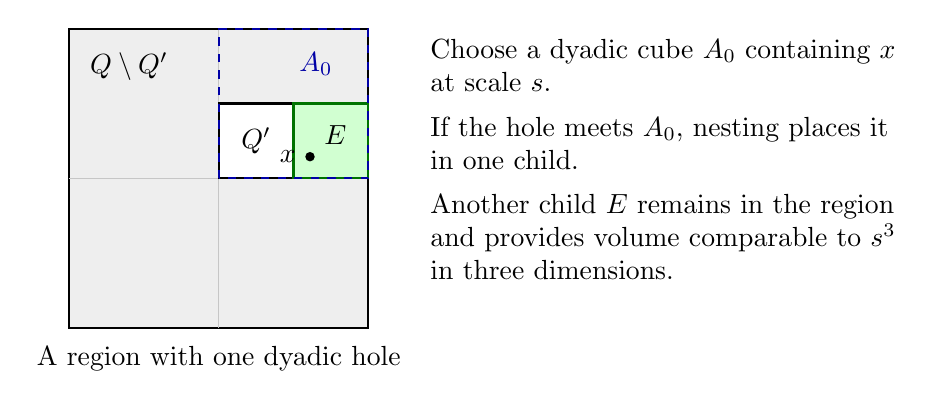
\begin{tikzpicture}[scale=0.95]
 \fill[gray!13] (0,0) rectangle (4,4);
 \draw[thick] (0,0) rectangle (4,4);
 \draw[gray!45] (2,0)--(2,4) (0,2)--(4,2);
 \fill[white] (2,2) rectangle (3,3);
 \draw[thick] (2,2) rectangle (3,3);
 \fill[green!18] (3,2) rectangle (4,3);
 \draw[green!45!black,thick] (3,2) rectangle (4,3);
 \draw[blue!65!black,dashed,thick] (2,2) rectangle (4,4);
 \fill (3.22,2.29) circle (1.8pt);
 \node[anchor=east] at (3.16,2.29) {$x$};
 \node at (2.5,2.5) {$Q'$};
 \node at (3.56,2.58) {$E$};
 \node[blue!65!black] at (3.3,3.53) {$A_0$};
 \node at (0.8,3.5) {$Q\setminus Q'$};
 \node[anchor=north] at (2,-0.12) {A region with one dyadic hole};
 \node[align=left,anchor=west,text width=6.0cm] at (4.7,2.25)
 {Choose a dyadic cube $A_0$ containing $x$ at scale $s$.\\[4pt]
  If the hole meets $A_0$, nesting places it in one child.\\[4pt]
  Another child $E$ remains in the region and provides volume
  comparable to $s^3$ in three dimensions.};
\end{tikzpicture}
\caption{A two-dimensional illustration of the thickness argument in
Lemma~\ref{mot:partition}.  The volume estimate is proved for
three-dimensional cubes.  It holds near the hole as well as near the
outer boundary, and survives every rigid motion.  This makes the
packing argument independent of the depth of the dyadic subdivision.}
\label{mot:partition-figure}
\end{figure}

\FloatBarrier

\subsection{Counting prescribed images of rich lines}

We give the two elementary geometric facts needed for the line-type
contributions.  In the first lemma a line-match weight is the full
number of source points on the specified line mapped to target
points on its specified image line.

\begin{lemma}[Two prescribed line images]
\label{mot:line-images}
Let \((L_1,L_2)\) and \((L'_1,L'_2)\) be ordered pairs of distinct
affine lines in \(\mathbb R^3\).
\begin{enumerate}
\item If the source lines are nonparallel, at most eight rigid
motions map \(L_i\) onto \(L'_i\) for \(i=1,2\).
\item If the source lines are parallel, the target lines must be
parallel at the same positive separation.  There are at most four
possible orthogonal linear parts, and for each one the admissible
translations form one affine line parallel to the target lines.
If all four lines contain at most \(H\) points of their respective
clouds, then
\begin{equation}
\label{mot:parallel-weight}
 \sum_g w_1(g)w_2(g)\le4H^3,
\end{equation}
where only motions with positive product are included.  That set
of motions is finite.
\end{enumerate}
Both conclusions allow both orientation classes.
\end{lemma}

\begin{proof}
For nonparallel lines choose unit directions \(a_1,a_2\) and
\(b_1,b_2\).  The orthogonal part \(S\) of a motion must satisfy
\(Sa_i=\varepsilon_i b_i\), with
\(\varepsilon_i\in\{1,-1\}\).  There are at most four sign
choices.  Each compatible choice determines the isometry on the
two-dimensional span of \(a_1,a_2\), and there are at most two
choices on its perpendicular line.  For each resulting \(S\),
the condition on its translation \(h\) imposed by each line is
an affine line in translation space with direction \(b_i\).
Those two affine lines are nonparallel, so their intersection
has at most one point.  This proves the bound of eight, whether
the original lines intersect or are skew.

For parallel lines choose unit directions \(a,b\).  Let \(d\)
be the nonzero perpendicular separation vector from \(L_1\) to
\(L_2\), and let \(e\) be the analogous vector for the ordered
target pair.  Orthogonality forces
\[
 Sa=\pm b,\qquad Sd=e.
\]
These equations determine \(S\) on a two-dimensional space,
with at most two choices on its perpendicular line.  There are
therefore at most four orthogonal parts in total.  For any fixed
one, mapping the first source line onto the first target line
fixes the translation modulo a scalar multiple of \(b\); the
second-line condition is then either impossible or automatically
satisfied.  This proves the geometric assertion.

Parametrize one such translation family by a real number \(\tau\).
Each pair of a source sample point on \(L_1\) and a target sample
point on \(L'_1\) determines a unique \(\tau\).  Thus
\[
 \sum_\tau w_1(\tau)
 \le |X\cap L_1|\,|Y\cap L'_1|\le H^2,
 \qquad w_2(\tau)\le H.
\]
Only finitely many \(\tau\) have positive first weight.  The
product sum for this linear part is at most \(H^3\); summing over
at most four parts proves \eqref{mot:parallel-weight}.  This
argument sums the actual translations and introduces no
discretization of the continuous family.
\end{proof}

\begin{lemma}[Parallel pairs at a fixed separation]
\label{mot:parallel-pairs}
Let \(\mathcal L\) be a finite family of at most \(L\) distinct
lines in \(\mathbb R^3\).  For each \(\rho>0\), the number of
ordered parallel pairs in \(\mathcal L\) at separation \(\rho\)
is \(O(L^{3/2})\), with an absolute implicit constant.
\end{lemma}

\begin{proof}
In one parallelism class of size \(q\), intersect the lines with
the plane through the origin perpendicular to their common
direction.  Their intersection points are distinct, and line
separation equals the Euclidean distance of these points.
Form the graph whose edges join points at distance \(\rho\).
Two different vertices have at most two common neighbors, because
two distinct circles of radius \(\rho\) have at most two common
points.  If the graph has \(e\) edges and degrees \(d_z\), then
\[
 \sum_z\binom{d_z}{2}\le2\binom q2,
 \qquad
 (2e)^2\le q\sum_zd_z^2\le3q^3.
\]
In the last inequality we used the preceding bound and
\(2e\le q(q-1)\).  Hence there are \(O(q^{3/2})\) ordered
pairs in this class.  Sum over the classes, using
\(\sum_jq_j^{3/2}\le(\sum_jq_j)^{3/2}\le L^{3/2}\).
\end{proof}

\subsection{Proof of the very-rich-motion estimate}

\begin{proof}[Proof of Theorem~\ref{mot:rich}]
We prove the stronger assertion stated at the start of the section.
Let \(X,Y\) be
clouds of at most \(N\) points, put \(A=N^{2/3}\), and suppose
that each line contains at most \(2A\) points of either cloud.
Write \(k_g=k_g(X,Y)\) throughout this proof.  We prove
\eqref{mot:rich-sum} with this notation.  This implies
the asserted result by \eqref{mot:physical-line-cap}.  Alternatively,
the claim for a congruent copy follows by composing the motions
with the inverse of the congruence, which preserves their match
counts and bijects the two orientation classes as appropriate.

Fix the absolute constants
\[
 \alpha=\frac1{14},\qquad
 \beta=\frac1{4K_{\mathrm{part}}},\qquad
 \nu=\frac{\eta_1}{4}.
\]
Choose \(C_{\mathrm{rich}}\) sufficiently large that
\begin{equation}
\label{mot:constant-choices}
 C_{\mathrm{rich}}>4,\qquad
 \frac\beta4 C_{\mathrm{rich}}^{9/14}
      \ge C_{\mathrm{loc}},\qquad
 \eta_1\beta C_{\mathrm{rich}}^{3/7}\ge1,\qquad
 \nu C_{\mathrm{rich}}\ge4.
\end{equation}
All constants on the right have already been fixed.  These choices
are independent of \(N\) and of the clouds.

Every motion with at least \(C_{\mathrm{rich}}A\) matches has a
noncollinear matched triple, because the line cap is \(2A\).
The finite choice of source and target ordered triples and the
at-most-two extensions per triple prove finiteness of the motion
set in the sum.  In particular, possible continuous families of
motions fixing a line are below the threshold unless they have
additional noncollinear matches, in which case this same finite
triple argument applies.

Bucket the high motions by
\[
 k\le k_g(X,Y)<2k,\qquad
 k=tA,\qquad t=2^jC_{\mathrm{rich}}\le N^{1/3}.
\]
If no such \(t\) exists, the sum is empty.  In a nonempty bucket
set
\begin{equation}
\label{mot:subdivision-parameters}
 r=t^{1+\alpha},\qquad
 m=8N/r,\qquad
 b=\beta k/r=\beta A t^{-\alpha}.
\end{equation}
Since \(t\le N^{1/3}\) and \(\alpha<2\), we have
\(1\le r\le N\), so Lemma~\ref{mot:partition} applies to both
clouds.  It supplies at most \(19r\) regions in each partition,
each with at most \(m\) points.

For the partitions just chosen, put \(X_R=X\cap R\) and
\(Y_{R'}=Y\cap R'\).  The local count is
\(n_{R,R'}(g)=k_g(X_R,Y_{R'})\).  These counts sum to \(k_g\),
and at most \(K_{\mathrm{part}}r\) are nonzero.  By
\eqref{mot:region-discard}, discarding those below \(b\) removes
at most \(K_{\mathrm{part}}rb=k/4\) matches.  At least \(3k/4\)
matches remain.
Bucket each remaining local count into
\(\ell\le n_{R,R'}(g)<2\ell\), with \(\ell=2^i b\), and
use the line/planar/general classification of
Lemma~\ref{mot:local} for the clouds \(X_R,Y_{R'}\) in that local
bucket.  A single global motion may contribute different local types
in different region pairs.

The local lower threshold is valid, since
\begin{equation}
\label{mot:local-scale-check}
 \frac{b}{m^{2/3}}
 =\frac\beta4\,t^{(2-\alpha)/3}
 =\frac\beta4\,t^{9/14}
 \ge C_{\mathrm{loc}}.
\end{equation}
We shall also need the full-cloud rich-line threshold
\(q=\eta_1b\) to be at least \(\sqrt N\).  The inequality
\(t\le N^{1/3}\) gives \(N^{1/6}\ge t^{1/2}\), so
\begin{equation}
\label{mot:rich-line-scale}
 \frac{q}{\sqrt N}
 =\eta_1\beta N^{1/6}t^{-\alpha}
 \ge\eta_1\beta t^{1/2-\alpha}
 =\eta_1\beta t^{3/7}\ge1.
\end{equation}
In particular these rich lines contain at least two points in every
nonempty bucket.  One may also record the power margin
\(b\ge\beta N^{9/14}\), although only
\eqref{mot:rich-line-scale} is needed below.

\paragraph{Motions with substantial non-line-type mass.}
Let \(\mathcal G_0\) consist of the motions in the global bucket
whose retained local non-line-type counts have total at least
\(k/4\).  For a fixed region pair and a local richness bucket,
Lemma~\ref{mot:local} bounds the number of non-line-type motions
by \(K_{\mathrm{loc}}m^3/\ell^{3/2}\).  Their local match mass
is therefore at most \(2K_{\mathrm{loc}}m^3/\sqrt\ell\).
Summing the geometric series over \(\ell=2^i b\) gives
\(O(m^3/\sqrt b)\) for each fixed region pair.  The bound remains
valid after restriction to our global bucket.  There are at most
\((19r)^2\) possible region pairs, whence
\begin{equation}
\label{mot:nonline-mass}
 |\mathcal G_0|\,k^2
 \le C k r^2\frac{m^3}{\sqrt b}
 \le C' N^3\frac{k}{r\sqrt b}
 =C''N^3\sqrt A\,t^{-\alpha/2}
 =C''\frac{N^4}{A}\,t^{-1/28}.
\end{equation}
The equality \(N^3\sqrt A=N^4/A\) uses \(A=N^{2/3}\).

\paragraph{Motions whose retained mass is mostly line type.}
For every remaining motion, at least \(k/2\) retained matches
belong to line-type local buckets.  In each such region pair,
choose one source line containing at least \(\eta_1\ell\) of
its local matches, and retain those matches as assigned line
matches.  Since \(n_{R,R'}(g)<2\ell\), this retains at least
\(\eta_1/2\) of that local count.  Thus the assigned line-match
mass \(W_g\) satisfies
\[
 W_g\ge\nu k,\qquad \nu=\eta_1/4.
\]
A physical source point participates in at most one region-pair
count for a fixed motion.  Hence no assigned match is repeated.
Pool assignments belonging to the same full source line \(L\),
and write its weight as \(w_{g,L}\).  Its target line is necessarily
\(gL\), and
\begin{equation}
\label{mot:pooled-line-weights}
 \sum_Lw_{g,L}=W_g\ge\nu k,
 \qquad 0\le w_{g,L}\le2A.
\end{equation}
Every line appearing on either side contains at least
\(\eta_1b=q\) ambient sample points, because it was chosen in a
local bucket with \(\ell\ge b\).

Let \(\mathcal L_X,\mathcal L_Y\) be the full lists of these
\(q\)-rich lines of the two clouds.  These are finite lists of
spanned lines.  Equations~\eqref{mot:st-rich} and
\eqref{mot:rich-line-scale} imply
\begin{equation}
\label{mot:rich-line-number}
 |\mathcal L_X|,|\mathcal L_Y|
 \le C\left(\frac{N^2}{q^3}+\frac Nq\right)
 \le C'\frac Nb.
\end{equation}
Denote a common upper bound in \eqref{mot:rich-line-number} by
\(L_*=C'N/b\).

The diagonal weights can be removed without losing a fixed
fraction.  Indeed, by \eqref{mot:constant-choices} and
\eqref{mot:pooled-line-weights},
\(W_g\ge\nu k\ge4A\).  Consequently
\begin{equation}
\label{mot:distinct-line-pair-mass}
 \sum_{L_1\ne L_2}w_{g,L_1}w_{g,L_2}
 =W_g^2-\sum_Lw_{g,L}^2
 \ge W_g^2-2AW_g
 \ge\tfrac12\nu^2 k^2.
\end{equation}

Sum this quantity over the remaining motions.  For nonparallel
source line pairs, there are at most \(L_*^4\) prescriptions of
an ordered source pair and its ordered target pair.  By
Lemma~\ref{mot:line-images}, each prescription has at most eight
motions, and each product of weights is at most \((2A)^2\).
Their total contribution is thus \(O(A^2L_*^4)\).

For a parallel ordered source pair, fix its positive separation
\(\rho\).  Lemma~\ref{mot:parallel-pairs} gives at most
\(O(L_*^{3/2})\) ordered target pairs at that separation, including
all target parallelism classes.  There are at most \(L_*^2\)
source pairs.  For every prescription, the pooled selected weights
are bounded by the full line-match weights in
Lemma~\ref{mot:line-images}; with \(H=2A\), its bound is
\(O(A^3)\).  Therefore the total parallel contribution is
\(O(A^3L_*^{7/2})\).

If \(\mathcal G_1\) denotes the remaining motions, the two cases
and \eqref{mot:distinct-line-pair-mass} give
\begin{equation}
\label{mot:line-mass}
 |\mathcal G_1|\,k^2
 \le C\left(A^2(N/b)^4+A^3(N/b)^{7/2}\right).
\end{equation}
This counts both orientations.  In the parallel case it sums the
whole continuous translation family through its finite positive
match support, rather than assuming a bounded number of motions
for the two prescribed lines.

\paragraph{Summing the global buckets.}
From \(b=\beta A t^{-\alpha}\), with its fixed positive
\(\beta\), the two terms in \eqref{mot:line-mass} are
\begin{align}
\label{mot:nonparallel-exponent}
 A^2(N/b)^4&=O\left(N^{8/3}t^{4\alpha}\right)
             =O\left(N^{8/3}t^{2/7}\right),\\
\label{mot:parallel-exponent}
 A^3(N/b)^{7/2}&=O\left(N^{19/6}t^{7\alpha/2}\right)
             =O\left(N^{19/6}t^{1/4}\right).
\end{align}
Summing these increasing geometric series up to
\(t\le N^{1/3}\) gives respectively
\[
 O\left(N^{58/21}\right)
 \quad\text{and}\quad
 O\left(N^{13/4}\right).
\]
Both are bounded by \(O(N^{10/3})=O(N^4/A)\); in fact they save
the powers \(N^{-4/7}\) and \(N^{-1/12}\), respectively.
The decreasing geometric series in
\eqref{mot:nonline-mass} gives
\[
 \sum_{j\ge0}
 O\left(\frac{N^4}{A}
       (2^jC_{\mathrm{rich}})^{-1/28}\right)
 =O(N^4/A).
\]
Finally \(k_g<2k\) in each global bucket, so replacing its
cardinality times \(k^2\) by the sum of the actual \(k_g^2\)
costs at most a factor of four.  The two types exhaust every
bucket, proving \eqref{mot:rich-sum}.
\end{proof}

\begin{remark}[Scope of the threshold and the deletion cost]
\label{mot:scope}
The finite line cap is essential for the sum over motions to make
sense.  For a collinear sample without such a high threshold,
infinitely many rotations about its containing line fix every
point.  In Theorem~\ref{mot:rich} each counted motion has a
noncollinear matched triple, which removes this issue.
For the reduction in this paper, \(M=o(A)\) guarantees the finite
hypothesis \(M\le A\) eventually.  Deleting every existing graph
edge whose endpoints are matches of the same motion above the threshold
costs at most \(\sum_g\binom{k_g}{2}=O(N^4/A)\).  Counting an edge for
several motions can only increase this upper bound.  In the proof of
Lemma~\ref{red:local-concentration}, the real Gram-matrix calculation
uses this deletion to bound the parameters in every local maximal
isotropic plane.
\end{remark}
